\section{System Design}
\label{sec:system}

In this section, we present the system design of \name to realize the two design choices presented in \Section\ref{sec:overview}.

\subsection{\name architecture}
\label{subsec:system:architecture}

\begin{figure}[htbp]
  \centering
  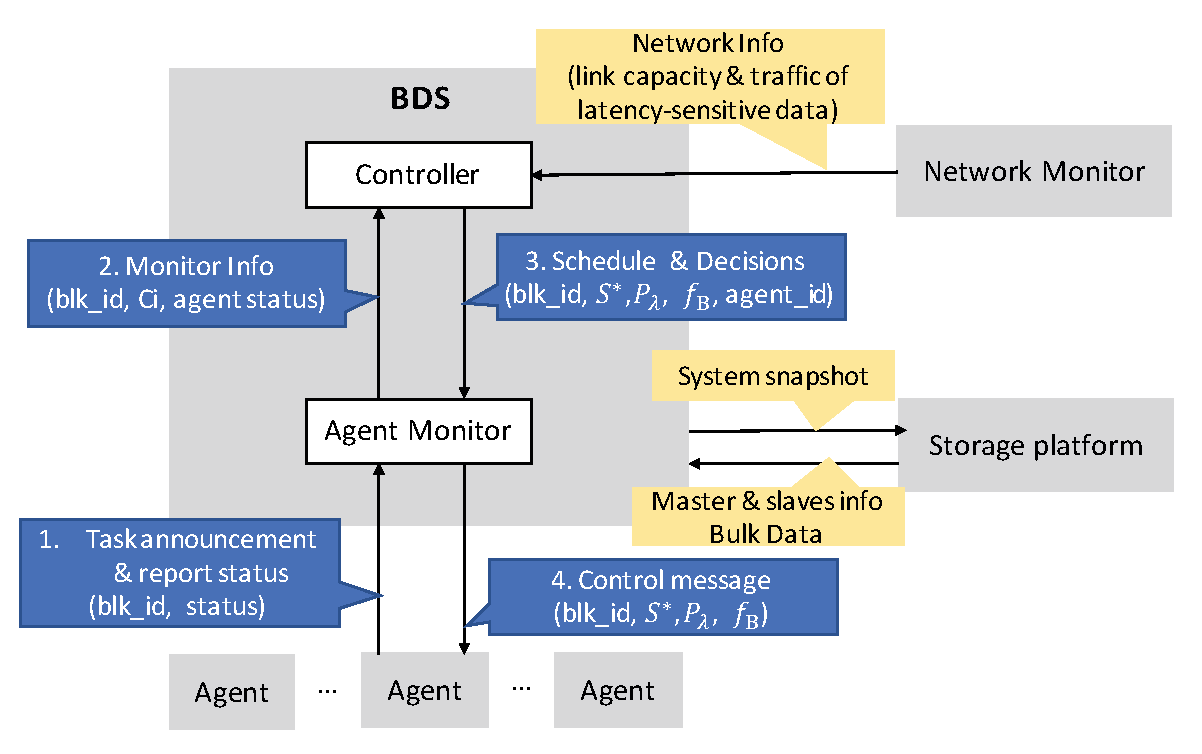
\includegraphics[width=3in]{images/implementation.eps}
  \caption{The implementation of \name.}
  \label{fig:implementation}
\end{figure}
%\vspace{-15pt}

\name reuses the same underlying multicast system described in \Section\ref{subsec:motivation:case-for}. Figure \ref{fig:implementation} shows the detailed architecture of \name. It consists of five components: Controller, Agent Monitor, Agent, Storage Platform, Network Monitor. (1) \emph{Controller} is a scheduler which executes the customized scheduling algorithm. (2) \emph{Agent Monitor} delivers messages between the \emph{Controller} and \emph{Agents}. (3) \emph{Agent} is a module deployed in each node. It announces the bulk data download requirement to the agent monitor and triggers the transmission. (4) \emph{Network Monitor} maintains each link's capacity and monitors the aggregated traffic of latency-sensitive data, which are the basic inputs of the scheduling algorithm. (5) \emph{Storage platform} records the system snapshot, including master and slave controller status, etc.

\subsection{Centralized control}
\label{subsec:system:centralized}

The centralized controller of \name sets a 3-second scheduling cycle and updates the scheduling results in each cycle. Specifically, the basic workflow in one cycle can be described as follows: (1) the local agent on each node checks the block status, records the id of blocks that finished downloading in this cycle, and then reports the completion information to the agent monitor in the form of two tuples \{blk\_id, status\}, by HTTP POST. (2) Agent Monitor aggregates the information from all the agents and send to the controller. (3) the controller runs the centralized scheduling algorithm, works out the near-optimal scheduling results ($s^*$, $p^*$, $f_{B_{i,j},p_\lambda}$), and then sends them to the agent monitor. (4) agent monitor then forwards the control messages back to the corresponding local agents by HTTP POST. (5) the local agent sets the transmission rate according to the received control message, then uses \emph{wget} tools to download the bulk data.

To make \name fault tolerant, the following scenarios are also considered. Firstly, what if the controller is not available? The controller is replicated three times for fault recovery. Once the master controller fails, one replica will be brought up via distributed consensus protocols, such as \cite{lamport1998part}. Secondly, what if a server is not available (or straggling)? If the agent on this server is still able to work, it will report the abnormal server state to the agent monitor. Otherwise, the other server that have selected this server as data source would report the invalid transmission situations to the agent monitor. In both cases, the controller would remove the server from the potential data sources in the next cycle scheduling. Thirdly, what if there is network partition between DCs or between DCs and the controller? If network partition happens between DCs and the controller, the whole network will work as a multi-tier peer-to-peer (MTP2P) network. If network partition happens between DCs, the DCs that locate in the same partition with the controller will work the same as before, while the separated DCs will downgrade to a MTP2P network.

There are two further optimizations.
\begin{itemize}
\item \emph{Merging blocks}. \name merges the blocks with the same source and destination pair $(s,d)$ into one subtask. There are two objectives. The first one is to reduce the computation scale and the second one is to achieve higher-efficient transmissions. Without this merging process: 1) there will be a large number of pending tasks in the next scheduling cycle, making calculation computationally hard to finish within an acceptable time; 2) all blocks will establish their connections at the same time, sharing the limited server rate, thus cannot be finished and will be hung up for the next cycle, resulting in inefficient transmissions.% To merge two blocks together, we should check all the three links in their corresponding $p^*$: the link between the source IDC and its corresponding super core, the combined cross-DR link, and the link between the destination IDC and the corresponding super core. Only when all the three links are matched, can we merge two blocks together. Earlier in Section \ref{P1}, the newly arrived task is split into blocks. After this merging procedure, some blocks are merged into subtasks, so in the next scheduling cycle, these subtasks will wait to be scheduled together with newly arrived tasks. The complete pseudo algorithm of BeSmart is shown in Algorithm \ref{BeSmart}.
\item \emph{Non-blocking update}. No matter how fast the controller runs, it still takes some time (e.g., $\delta t$) to work out the near-optimal scheduling solutions in each cycle. During this algorithm running time, \name continues the transmissions according to the configurations in the last cycle instead of pausing transfers and waiting for new configurations. To ensure consistency, the controller will estimate the task status after $\delta t$ and use this future status as inputs of the scheduling algorithm.
\end{itemize}

%\begin{itemize}
%
%\item Start with the basic workflow of each 3-second cycle: (1) how local agent collects delivery status, (2) send messages to the controller, (3) controller runs the algorithm, (4) control message to each local agent, and (5) how local agent enforce decision.
%
%\item Fault tolerance: what if a server is not available (or straggling), what if one controller instance is not available, what if there is network partition between DCs or between DCs and the controller.
%
%\item Explain two optimizations:
%\begin{itemize}
%\item Merging blocks
%\item Non-blocking update
%\end{itemize}
%
%\end{itemize}

\subsection{Dynamic bandwidth separation}
\label{subsec:system:separation}

To guarantee dynamic bandwidth separation between background data and the delay-sensitive user data, \name monitors the real-time size of latency-sensitive traffic by the network monitor component, which monitors the traffic from different IPs, thus can calculate the aggregated traffic on all the inter-/intra-DC links.

With the known link capacity and the aggregated size of latency-sensitive traffic, the residual bandwidth for background data can then be calculated by the difference of the two. Thus, the upper limit for the available bandwidth of all links are all conformed in the scheduling algorithm.

Finally, each agent in the server end enforces the bandwidth limits by Linux Traffic Control (TC). So far, \name achieves the bandwidth separation dynamically and in real-time.

%
%\begin{itemize}
%
%\item First, how to get real-time aggregated size of latency-sensitive traffic.
%
%\item Second, how to calculate the bandwidth cap for background bulk traffic
%
%\item Finally, how to enforce the bandwidth cap.
%
%\end{itemize}



